\documentclass[a4paper,10pt]{article}
%\documentclass[a4paper,10pt]{scrartcl}

\usepackage[utf8]{inputenc}
\usepackage{polski}
\usepackage[polish]{babel}
\usepackage{hyperref}
\usepackage{graphicx}


\title{Dokumentacja projektu z Baz Danych: System Zarządzania Partią Polityczną}
\author{Filip Marcinek}
\date{semestr letni 2019}

\begin{document}
\maketitle

Specyfikacja projektu jest dostępna pod linkiem: \href{https://github.com/piotrekiiuwr/bd2019-projekt/blob/master/projekt.md}{https://github.com/piotrekiiuwr/bd2019-projekt/blob/master/projekt.md}.

\section{Uruchomienie programu}
Program uruchamia się poprzez uruchomienie skryptu \texttt{run.sh} z odpowiednimi parametrami (jak w dokumentacji) oraz przekierowanie na jego standardowe wejście pliku z instrukcjami API (sformatowanymi jak w dokumentacji).
Program musi być uruchomiony w tym samym katalogu, w którym znajduje się baza danych, którą obsługuje (baza danych powinna istnieć przed pierwszym uruchomieniem programu).
Flagi inne niż wspomniane w dokumentacji są ignorowane przez program. Jeżeli program dostanie instrukcje API w nieprawidłowym formacie - zwróci błąd. \\
Przykładowe uruchomienie programu: \texttt{./run.sh --init < init-test.json}.

\section{Projekt bazy danych}
Projekt składa się z dwóch modułów:
\begin{itemize}
 \item pythonowego programu, który parsuje wejście, wysyła żadania do bazy danych oraz odbiera je, przetwarza i wyświetla,
 \item bazy danych sql, w której zaimplementowane są wszystkie funkcjonalności API i przechowywane dane przekazywane do programu.
\end{itemize}

\begin{figure}
  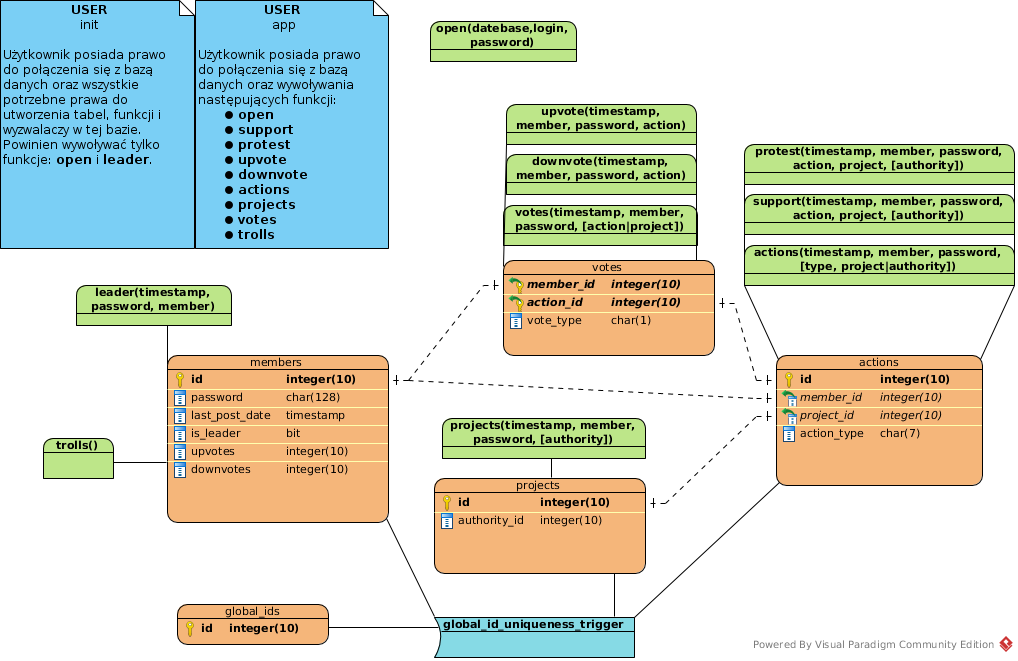
\includegraphics[width=\linewidth]{Projekt_bazy_danych_2019_Filip_Marcinek.png}
  \caption{Projekt bazy danych}
  \label{fig:project}
\end{figure}

Rysunek 1. przedstawia projekt bazy danych, na którym możemy zobaczyć uprawnienia użytkowników, tabele oraz ogólny model triggerów i funkcji wykorzystywanych przez użytkowników.
Warto zauważyć, że użytkownik \texttt{app} ma prawo tylko do wywoływania funkcji sql wymienionych w dokumentacji i nie jego kompetencje nie wykraczają poza ten obszar.
Trigger \texttt{global\_id\_uniqueness\_trigger} używany jest do zachowania warunku unikalności wszystkich id w bazie danych. Funkcje połączone są liniami z tabelami, które wykorzystują w głównej mierze.

\newpage

\section{Implementacja}
\indent Pythonowy program wykorzystuje bibliotekę \texttt{psycopg2} do łączenia się z bazą danych. Baza danych sql tworzy użytkownika \texttt{app} ze wspomnianymi wcześniej prawami oraz tabele, triggery i funkcje przedstawione ogólnie w sekcji \textit{Projekt bazy danych}. \\
\indent Unikalność wszystkich id w bazie danych jest zachowana z wykorzystaniem tabeli \texttt{global\_ids}, do której za pomocą triggerów wstawiane jest każde id nowego obiektu w bazie (jeżeli któreś id się powtórzy wystąpi błąd naruszenia własności klucza w \texttt{global\_ids}). \\
\indent Hasła użytkowników są haszowane z pomocą modułu \texttt{pgcrypto} i przechowywane w tabeli \texttt{members}, w której znajdują się także id użytkowników, flaga \texttt{is\_leader} -- czy użytkownik jest liderem partii, \texttt{last\_post\_date} -- data ostatniego posta użytkownika, liczniki \texttt{upvotes} i \texttt{downvotes} -- liczby głosów (za i przeciw) oddanych na ich akcje. \\
\indent Przy każdym poprawnym działaniu w polu \texttt{last\_post\_date} zapisywana jest data tego działania (dla funkcjonowania bazy zgodnie ze specyfikacją wystarczy przechowywanie daty ostatniego działania użytkownika). \\
\indent Funkcje \texttt{support} i \texttt{protest} wstawiają akcje do tabeli \texttt{actions} z oznaczeniem 'support'/'protest' w kolumnie \texttt{action\_type}, a projekty wraz z odpowiadającymi im organami władzy do tabeli \texttt{projects}. \\
\indent Funkcje \texttt{upvote} i \texttt{downvote} zapisują oddane głosy w tabeli \texttt{votes} wraz z oznaczeniem 'u'/'d' (upvote/downvote) w kolumnie \texttt{vote\_type}. \\
\indent Pozostałe funkcje wymagają praw lidera partii (flaga \texttt{is\_leader}), co jest sprawdzane przed wszelkimi modyfikacjami czy odczytami z bazy przez użytkownika (podobnie przed wykonaniem zadania funkcji API, najpierw sprawdzane jest, czy użytkownik nie jest zamrożony, poprzez porównanie aktualnej daty z datą ostatniego działania użytkownika). \\
\indent Funkcja \texttt{actions} wykorzystuje pomocniczą funkcję (dla czytelności kodu) i obsługuje wszystkie przypadki wymienione w specyfikacji.
Funkcji \texttt{projects} wystarcza korzystanie z samej tylko tabeli \texttt{projects}. \\
\indent Funkcja \texttt{trolls} w prosty sposób wykorzystuje kolumny \texttt{last\_post\_date, upvotes} i \texttt{downvotes} z tabeli \texttt{members}.


\end{document}
